Having described how to operate with basic sets, we consider a more fundamental representation problem.
%
We have seen that there exist classes of sets.
Some of them, such as polyhedra, are closed under various set operations. That property is convenient because the type of the result is known in advance.
%
The whole class of convex sets is also closed under the operations described in the upper part of Table~\ref{tab:operations}, but we can typically not represent the result with the limited amount of set types in LazySets. This is not a shortcoming of LazySets: you would need infinitely many set representations for all possible combinations! However, we can resort to a simple yet powerful trick to effectively represent the result of the set operations: \emph{lazy representation}.
%
Going a step further, by making both basic set types and operations between sets live in the same abstraction layer (namely always subtyping \code{LazySet} irrespective whether it is a concrete set or the result of an operation) allows to easily \emph{compose} set computations.


\subsection{Type composition} \label{sec:composition}

To give an example, the Minkowski sum of a square and a disc (two-dimensional balls in the infinity norm and Euclidean norm) is not representable with a basic type in LazySets. Hence \code{minkowski\_sum} will yield an error. But we can apply the \emph{lazy} operation, which is called \code{MinkowskiSum}. \code{MinkowskiSum} itself subtypes \code{LazySet}. This choice allows for ease of composition.

We wrap the operands in a new object that, by definition, represents the result of the operation, but without actually performing the computation. (This also motivates the name of LazySets).

\smallskip

As an illustrative example, suppose that we are interested in the formula $\Omega_0 = \CH(\X_0, \Phi \X_0 \oplus Y)$, where $\CH$ and $\oplus$ are defined in Table~\ref{tab:operations}, $X_0$ and $Y$ are sets, and $\Phi$ is a matrix defined in Appendix~\ref{sec:omega0}. Such formulas are prevalent in reachability analysis of linear initial-value problems, or nonlinear ones after some form of conservative linearization; see for example \cite{althoff2020set,ForetsS21} and references therein. Given the sets $\X_0$, $Y$, and the matrix $\Phi$, we can write:

\begin{minipage}{\linewidth}
\begin{lstlisting}
julia> Ω₀ = CH(X₀, Φ*X₀ ⊕ Y)
\end{lstlisting}
\end{minipage}

\begin{minipage}{0.69\linewidth}
Then, $\Omega_0$ is a (nested) \emph{lazy} representation of the  operation just as a normal \code{LazySet}. As such, it can be used for further operations (conversion, approximation, evaluation). The structure of the nested operations is internally represented in the form of a tree, which can be visualized with \href{https://github.com/JuliaTeX/TreeView.jl}{TreeView.jl} as shown in the diagram (right).
\end{minipage}
\hfill
\begin{minipage}{0.2\linewidth}
	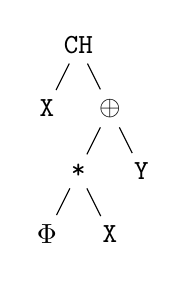
\begin{tikzpicture}[level/.style={sibling distance=8mm,level distance=8mm}]
		\node {\texttt{CH}}
		child {
			node {\texttt{X}}
		}
		child {
			node {$\oplus$}
			child {
				node {\texttt{*}}
				child {
					node {$\Phi$}
				}
				child {
					node {\texttt{X}}
				}
			}
			child {
				node {\texttt{Y}}
			}
		};
	\end{tikzpicture}
\end{minipage}

\smallskip

Lazy operations can be efficiently evaluated, as we describe next.


\subsection{Support-function calculus} \label{sec:supfun}

A standard approach to operate with compact and convex sets $\X \in \R^n$ is to use the \emph{support function} \cite{LeGuernic09}.
%
The support function along direction $d \in \R^n$, denoted $\rho(d, \X)$, is the maximum of $d^T x$ over all $x \in \X$, i.e., the support function describes the (signed) distance of the supporting hyperplane in direction $d$ from the origin.
%
It can be used to efficiently find the boundary of a set in a given direction.
%
The maximizers are called \emph{support vectors} $\sigma(d, \X)$. Intuitively, the support vectors are the extreme points of $\X$ in direction $d$.
%
Basic properties of the support function are given in Appendix~\ref{sec:supfunc_properties}.

For various set representations, the support function is known analytically and can be efficiently evaluated numerically. Such cases include hyperrectangular sets and zonotopic sets.
%
For sets with less structure, e.g., if $\X$ is a polytope in half-space representation, its support function can be computed by solving a linear program, for which fast and robust solvers exist.
%
But the main advantage of using the support function in LazySets lies in the extensive use of \emph{composition rules}, as we describe later.

\smallskip

LazySets offers \code{$\uprho$(d, X)} (or \code{support\_function(d, X)}) to compute the support function $\rho(d,\X)$, and \code{$\upsigma$(d, X)} (or \code{support\_vector(d, X)}) to compute (some) support vector $\sigma(d,\X)$. Fig.~\ref{fig:supfunc} (left) illustrates the evaluation of the support function over the polygon $\X$ (orange) along direction $(-1, 1)^T$.

\begin{minipage}{\linewidth}
\vspace{-\abovedisplayskip}
\begin{lstlisting}
julia> d = [-1, 1]

julia> ρ(d, X) # or support_function(d, X)
3.6

julia> σ(d, X) # or support_vector(d, X)
[-3.0, 0.6]
\end{lstlisting}
\end{minipage}

\begin{figure}
	\centering
	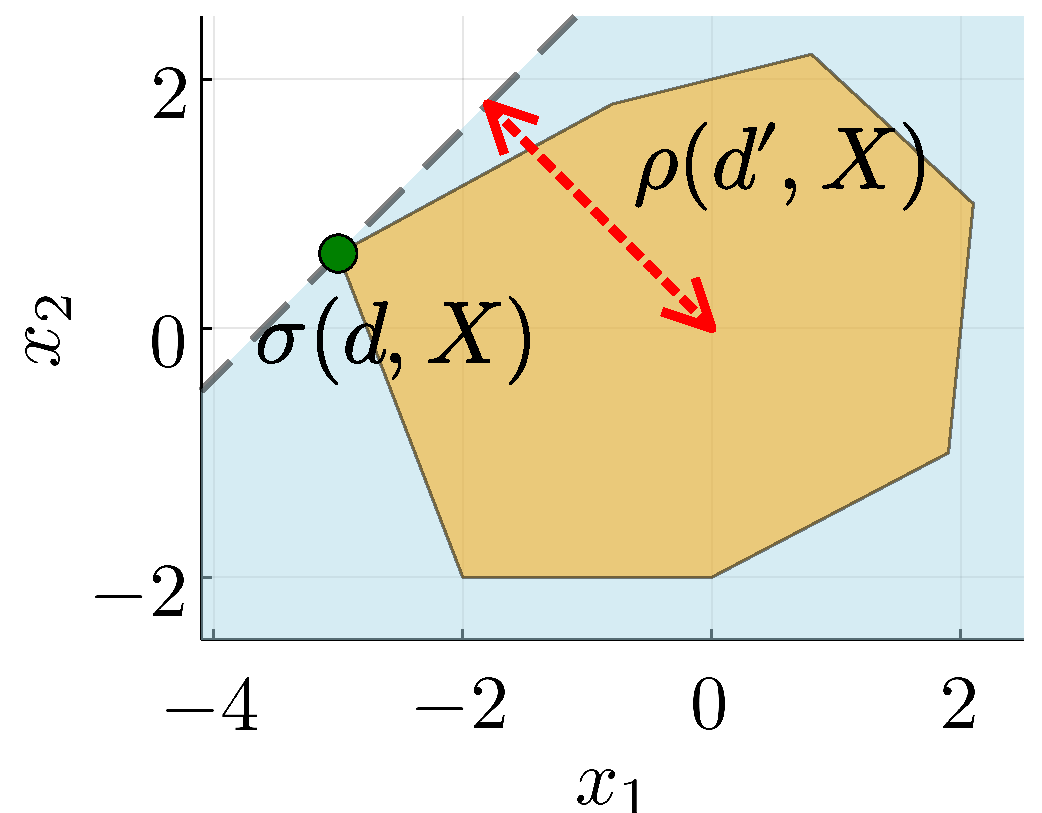
\includegraphics[width=0.49\linewidth, keepaspectratio]{img/supfunc}
	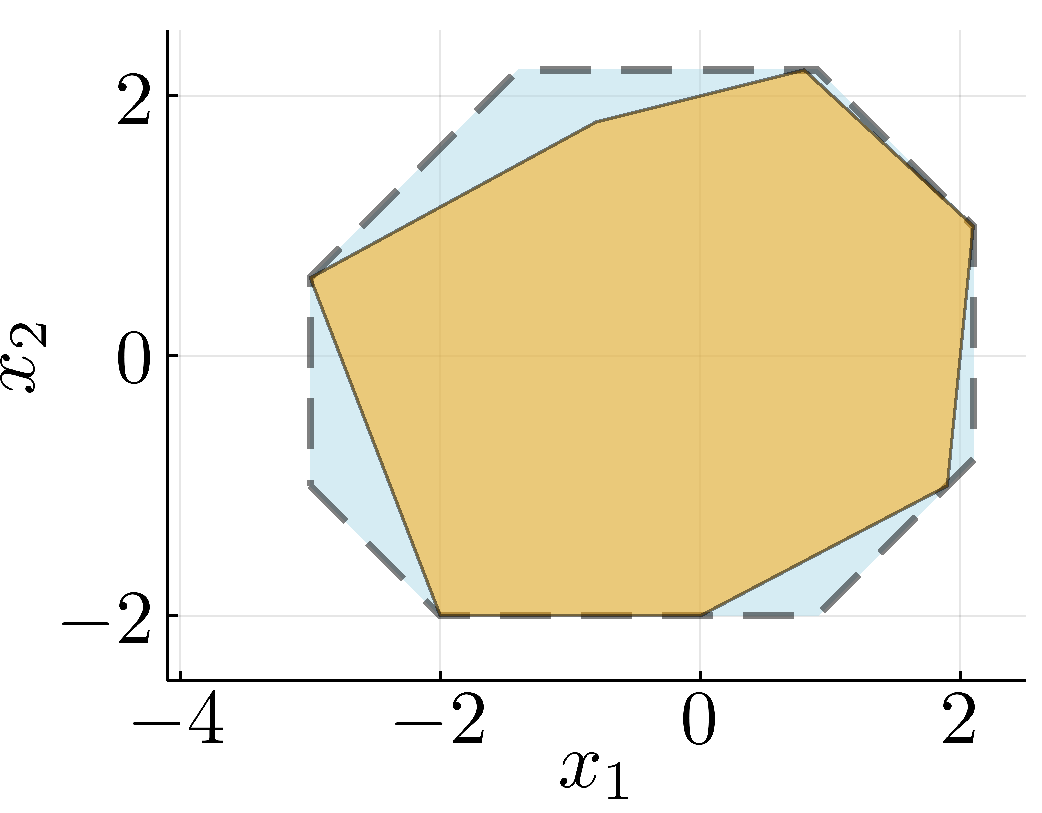
\includegraphics[width=0.49\linewidth, keepaspectratio]{img/supfunc_oct}
	\vspace*{1mm}
	\caption{Left: The supporting hyperplane of the set $\X$ along direction $d$.
	In red we plot the distance of the hyperplane to the origin, which is given by $\rho(d', \X)$ where $d' = d / \Vert d \Vert$.
	Right: An outer approximation of $\X$ using the eight directions of a regular octagon.}
	\label{fig:supfunc}
\end{figure}

Consider again the set $\Omega_0$ from the previous section. Suppose that we are interested in the support value of $\Omega_0$ along a given direction $d \in \R^2$.
%
Since the support function distributes over the Minkowski sum, $\rho(d, \X \oplus \Y) = \rho(d, \X) + \rho(d, \Y)$ for any pair of sets $\X, \Y \subseteq \R^n$, and since it holds that $\rho(d, M \X) = \rho(M^T d, \X)$ for any matrix $M \in \R^{n \times n}$, we can propagate the computation through the operation tree until a concrete set is found, and in many cases, an analytic formula is available.
%
That is precisely what LazySets does, automatically, when we make queries to the lazy set such as asking for its support function along $d = (-1, 1)^T$ from before.

\begin{minipage}{\linewidth}
	\vspace{-\abovedisplayskip}
	\begin{lstlisting}
julia> @btime ρ($d, $Ω₀)
117.236 ns (2 allocations: 192 bytes)
-0.8

julia> @btime ρ($d, concretize($Ω₀))
  23.700 μs (203 allocations: 16.03 KiB)
-0.8
	\end{lstlisting}
\end{minipage}

In the first benchmark we evaluate the support function on the lazy set.\footnote{The Julia macro \code{@btime} provided by the \href{https://github.com/JuliaCI/BenchmarkTools.jl}{BenchmarkTools.jl} package evaluates the given command multiple times and returns the smallest record.}
In the second benchmark we first convert to a concrete set representation (in this case a polygon in vertex representation) and then evaluate the support function.
The first case is two orders of magnitude faster.
This exemplifies that set computations can be implemented efficiently using the support function, which becomes more prominent in higher dimensions.

We note that in the above computation we have only obtained a bound in direction $d$, not in other directions. For many applications it is sufficient to evaluate the support function in only a few directions. For example, in the helicopter model presented in Section~\ref{sec:reachability} we are only interested in the vertical velocity, so we only need to evaluate the support function twice to obtain the upper and lower bound in that dimension.
Another example is to enclose $\Omega_0$ with a bounded set, for which we can pick a list of \emph{template} directions (see Section~\ref{sec:approximation}).
